\documentclass[12pt, titlepage]{article}

\usepackage{graphicx}
\usepackage{booktabs}
\usepackage{tabularx}
\usepackage{hyperref}
\hypersetup{
    colorlinks,
    citecolor=black,
    filecolor=black,
    linkcolor=black,
    urlcolor=blue
}
\usepackage[round]{natbib}

\title{SE 3XA3: Software Requirements Specification\\Scrabble}

\author{Team \#214, The Trifecta
		\\Kanakabha Choudhri, choudhrk
		\\ Raymond Tu, tur1
		\\ Lucia Cristiano, cristial
}

\date{February 9, 2020}

%\input{../Comments}

\begin{document}

\maketitle

\pagenumbering{roman}
\tableofcontents
\listoftables
\listoffigures

\begin{table}[bp]
\caption{\bf Revision History}
\begin{tabularx}{\textwidth}{p{3cm}p{2cm}X}
\toprule {\bf Date} & {\bf Version} & {\bf Notes}\\
\midrule
Jan. 24, 2020 & 1.0 & Adding names and introduction\\
Feb. 1, 2020 & 1.0 & Added to Project Drivers, FRs, NFRs, Project Issues\\
\bottomrule
\end{tabularx}
\end{table}

\newpage

\pagenumbering{arabic}
This document describes the requirements for the Scrabble project created by The Trifecta. This document will explain the scope and the requirements of the project in an many that can be easily understood by stakeholders and developers working on the project.

The template for the Software Requirements Specification (SRS) is a subset of the Volere template~\cite{robertson_robertson}. Any modifications to this template will be mentioned in the appendix.
\section{Project Drivers}

\subsection{The Purpose of the Project}
The purpose of the this project is to modify a a text based version of the board game version Scrabble to include a Graphical User Interface (GUI). As well as re-implement the code to modular rather a monolithic piece of software and follow a set of formal documentation. 
\subsection{The Stakeholders}
\subsubsection{The Client}
    The clients are any user who wishes to play online scrabble. The clients will consist of individuals who enjoy board games, such as Scrabble, and have a desire to play these game digitally. 
\subsubsection{The Customers}
    The customers of this project are our professor Dr.Asghar Bokhari and our
    teaching assistants (TAs) Andrew Lucentini and Hosseinkord Maryam. This group of individuals will inform the progress of the project based on feedback.
\subsubsection{Other Stakeholders}
    Other stakeholders include the original author of the repository, fayrose, and other Github users who have forked the project. They have a desire to see the project succeed and improve, these features can then either be applied to their own projects or built upon.
    
\subsection{Mandated Constraints}
    The main constraint for the project is the time constraint, the project must be completed by April 6, 2020. The system constraint is that the project must be run on a system with Python 3 installed. The space constraint is reliant on the system and it's hard drive space, but the project must take up reasonable amounts of memory on the hard drive. Additionally, the project will be constrained by the processing power of the system. Internet connection is not required so will not be a constraint for the system.

\subsection{Naming Conventions and Terminology}
\begin{table}[!htb]
    \centering
    \caption{Acronyms and Abbreviations}
    \begin{tabular}{|c|c|}
        \hline
        Acronym/Abbreviation & Full Form \\
        \hline
        SRS & Software Requirement Specification\\
        GUI & Graphical User Interface \\
        FR & Functional Requirements \\
        NFR & Non-functional requirement\\
        TA & Teaching Assistant\\
        MVC & Model-View-Controller\\
        \hline
    \end{tabular}
\end{table}

\begin{table}[!htb]
    \centering
    \caption{Definitions}
    \begin{tabular}{|c|c|}
        \hline
        Term & Definition \\
        \hline
        Tkinter & Open-source python library used to implement the GUI for the project. \\
        User & Player who will be playing the Scrabble project game. \\  
        Premium Squares & Represents a double or triple score multiplier for a word/letter. \\
        Crossword Fashion & Words on the board connect through a shared number of letters. \\
        \hline
    \end{tabular}
\end{table}

\subsection{Relevant Facts and Assumptions}
\begin{enumerate}
    \item It is assumed that the users have the visual and physical capabilities required to play the game.
    \item It is assumed that users know how to use a computer, since the software is played on a computer.
    \item It is assumed the users know the English language at a basic level.
    \item It is assumed that most users will have Windows/MacOS/Linux as the operating system on their computer to execute the software. 
    \item It is assumed that users do not need an internet connection once the game is installed into their computer as an executable file that they would only need to click to run.
    \item The users do not need prior gaming experience to play this game.
\end{enumerate}

%User characteristics should go under assumptions.

\section{Functional Requirements}

\subsection{The Scope of the Work and the Product} 

\subsubsection{The Context of the Work} %%KANAK
%
\begin{figure}[ht]
\centering
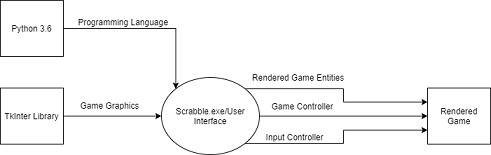
\includegraphics{srs_context_of_work.png}\\
\caption{Scrabble Context Diagram}
\end{figure}
\subsubsection{Work Partitioning} %%raymond -- stuff like business events
%

\begin{table}[!htb]
    \centering
    \caption{Work Partitioning}
    \begin{tabular}{|c|c|}
        \hline
        Event Name & Summary \\
        \hline
        Player places word & System checks if word exists in dictionary and if placement is valid.\\
        All tiles are played & System checks win state to see which player won. \\  
        Board is full & System checks win state to see which player won. \\
        Player exchanges tiles & System takes discarded tiles and randomly assigns new ones to player. \\
        \hline
    \end{tabular}
\end{table}

\subsubsection{Individual Product Use Cases}%Lucia
The main use case for the product consists of two to four users playing a game of scrabble. The users will use the letters given to them by the system to create words and place them on the board. The system will keep track of the players score until the game is completed. The player with the highest score wins the game.

\subsection{Functional Requirements}
\begin{enumerate} %raymond 1-4
    \item 
    Requirement Number: FR1 \\
    The system shall provide a user manual outlining the rules of the game. \\
    Rationale: A user manual will outline the rules of our implementation of Scrabble (different house rules exist) as well make it clear to the user how to play the game and use our GUI.\\
    \item 
    Requirement Number: FR2 \\
    The system shall display a game board size of is $BOARD\_WIDTHXBOARD\_HEIGHT$ and correct placement of premium squares. \\
    Rationale: The game board size stays consistent as well as consistent locations of premium squares to keep gameplay fair and consistent. Random generation of the board would open up the system to unbalanced gameplay and situations.\\
    \item 
    Requirement Number: FR3 \\
    The system shall request user to enter a number of players, between $MIN\_PLAYER$ and $MAX\_PLAYER$. \\
    Rationale: Because the system is entirely player vs player, there must be at least 2 players. The maximum number of players keeps our project within a reasonable scope. \\
    \item
    Requirement Number: FR4 \\
    The system shall allow user to enter a name for each player. \\
    Rationale: Having names for each player vs impersonal naming such as Player 1, 2, etc. will make it clear which player currently has their turn, as well makes score rankings more personal for the player.\\
    \item 
    Requirement Number: FR5 \\ %Lucia
    The system shall provide users with tiles not exceeding $MAX\_NUM\_TILES$.\\
    Rationale: The digital version of the game must follow the rules of the board game for consistency.\\
    \item 
    Requirement Number: FR6 \\
    The system shall check that user inputs to ensure that words are valid, based on English dictionary, and not shorter than $MIN\_NUM\_LETTERS$. \\
    Rationale: This prevents the user from typing gibberish and it still is accepted as a word. This is consistent with the board game rules, that use a dictionary to ensure if words are valid.\\
    \item 
     Requirement Number: FR7 \\
     The system shall inform user if their inputted word is invalid and prompt to try again.\\
     Rationale: This allows the user to know if their word is not allowed and gives them a chance to complete their turn.\\
    \item 
     Requirement Number: FR8 \\ %lucia
     The system shall allow user to place tile within dimension of game board, in horizontal and vertical orientation.\\
     Rationale: This simulates the act of placing a word down on a physical game board and is consistent with word placement in the board game.\\
    \item
    %%Rationale for 9-12 KANAK
    Requirement Number: FR9 \\
    The system shall ensure users place words in crossword fashion in relation to existing words on the board.\\
    Rationale: This acts as a limit on where and when words can be made which helps in the users decision making in the game.\\
    \item 
    Requirement Number: FR10 \\
    The system shall tally user's score based on letter tile values and placement on premium squares.\\
    Rationale: This is for both accurate scoring and motivation for a user to think of more creative words with the letters they have and/or the ones already on the board.\\
    \item 
    Requirement Number: FR11 \\
    The system shall hide each individuals set of letters from other players on the board.\\
    Rationale: This is for game fairness and adds an element of suspense which results in spontaneous thinking of words per turn.\\
    \item
    Requirement Number: FR12 \\
    The system shall end the game when no letter tiles remain in bag and one user has played all their tiles.\\
    Rationale: This acts as the final state of the game at which point game resources would have been used up.\\
\end{enumerate}

\section{Non-functional Requirements}

\subsection{Look and Feel Requirements}
\begin{enumerate}
    \item NFR Number: LF1\\ %%KANAK
    The system should give a warm, welcoming and homely feeling to the user that they would like to show to their families as well.\\
    Fit Criterion: The color schemes and overall layout must closely match environments and surroundings that are cognitively known to be warm and welcoming.
\end{enumerate}

\subsection{Usability and Humanity Requirements}
\subsubsection{Ease of Use Requirements}
\begin{enumerate}
    \item NFR Number: UH1\\ %%LUCIA
    The system shall be understood and playable by users of MIN\_AGE or older.\\
    Fit Criterion: Tests will be ran with users of MIN\_AGE, with 85\% reporting that they felt comfortable playing the game.
    \item NFR Number: UH2\\
    The interface of the system will have a consistent layout that is reminiscent of the Scrabble board game.\\
    Fit Criterion: 95\% of users will be able to correctly identify the game as scrabble after about MIN\_TIME seconds of gameplay. 
    \item NFR Number: UH3\\
    The user shall control the game using only the keyboard and the mouse.\\
    Fit Criterion: Tester will ensure that on keyboard and mouse is used during play of the Scrabble game.
\end{enumerate}
\subsubsection{Personalization and Internationalization Requirements}
N/A
\subsubsection{Learning Requirements}
\begin{enumerate}
    \item NFR Number: UH4\\ %%LUCIA
    The interface of the system shall be intuitive and can be learned without a tutorial.\\
    Fit Criterion: After playing a single game 85\% of users will state that they had no issues understanding how to navigate the game. 
    \item NFR Number: UH5\\ %%LUCIA
    The users shall remember how to navigate the interface after playing a single scrabble game. \\
    Fit Criterion: A test group will have users play the game two separate times a week apart. 90\% of the users will correctly control the game upon the second session. 
\end{enumerate}
\subsubsection{Understandability and Politeness Requirements}
\begin{enumerate}
    \item NFR Number: UH6\\ %%LUCIA
    The interface of the system shall include descriptive text that accurately describe the functionality of various items in the interface.\\
    Fit Criterion: After a single game 90\% of users will report little to no frustration when surveyed about their game experience.
     \item NFR Number: UH7\\ %%LUCIA
    The interface of the system shall include use common symbols to represent actions.\\
    Fit Criterion: After a single game 90\% of users will be able to recognize various symbols from the game.
\end{enumerate}
\subsubsection{Accessibility Requirements}
N/A

\subsection{Performance Requirements}
\begin{enumerate}
    \item NFR Number: PR1\\%%RAYMOND
    The system shall process turn changes within a reasonable time limit.
    Fit Criterion: The system check for a valid move will take no more than 10 seconds before the turn is changed or the user is prompted to give another move.
    \item NFR Number: PR2\\%%RAYMOND
    The system shall be in a playable state until the next major update.
    Fit Criterion: A questionnaire will be provided to confirm at least 90\% of users were able to use the software prior to the next major update.
\end{enumerate}

\subsection{Operational and Environmental Requirements}
\begin{enumerate} %%KANAK
    \item NFR Number: OE1\\
    The system should take a reasonable time to open up.\\
    Fit Criterion: The system shall not take more than 10 seconds to load and open up for the user to start playing the game.
    \item NFR Number: OE2\\
    The initial setup of the game should be within a reasonable time limit.\\
    Fit Criterion: The system shall take 20 minutes at most to fully download and install.
\end{enumerate}

\subsection{Maintainability and Support Requirements}
\begin{enumerate}
    \item NFR Number: MS1\\ %%RAYMOND
    The system shall be easily maintainable for future updates.\\
    Fit Criterion: A focus group of programmers will rate the maintainability of the system from 1-5.
    \item NFR Number: MS1\\ %%RAYMOND
    The system shall easily allow the implementation of new updates/features.\\
    Fit Criterion: Software design experts will be asked to rate the design of the system and if it allows for easy implementation of new features from a scale of 1-10.
    \item NFR Number: MS1\\ %%RAYMOND
    The system shall be operational until the next Python3 update.\\
    Fit Criterion: A questionnaire will be provided to confirm at least 90\% of users were able to use the software prior to the next major Python3 update.
\end{enumerate}

\subsection{Security Requirements}
N/A
\subsection{Cultural Requirements} %LUCIA
\begin{enumerate}
    \item NFR Number: CR1 \\
    The Scrabble project shall allow users to place words that are deemed culturally offensive or inappropriate.  \\
    Fit Criterion: The dictionary used by the Scrabble project to validate words will be reviewed by 5 users of various backgrounds for any culturally insensitive words.
    \item NFR Number: CR2\\
    The users of the Scrabble project can be of any cultural background as long as they have a basic understanding of the English language.\\
    Fit Criterion: The Scrabble project will be tested with 5 users at different levels of English language proficiency to ensure that a wide range of users can play the game. 
\end{enumerate}
\subsection{Legal Requirements}
\begin{enumerate}
    \item NFR Number: LR1 \\
    The application shall be under an open source license. \\
    Fit Criterion: An open source license shall be included in the project repository
\end{enumerate}

\subsection{Health and Safety Requirements} 
\begin{enumerate}
    \item NFR Number: HSR1\\
    The application shall include preventative measures against eye strain due to long playing periods.\\ 
    Fit Criterion: The application should include adequately sized text to improve readability, and use colour combinations that are pleasant to the eye. 
\end{enumerate}
% This section is not in the original Volere template, but health and safety are
% issues that should be considered for every engineering project.

\section{Project Issues}

\subsection{Open Issues}%raymond
%
The feasibility of the usage of Tkinter for the Front-end GUI implementation to connect with the backend is still in question. Additionally, the portability of the Tkinter GUI for example colours is still an issue for MacOS. Additionally, whether parts the existing Scrabble implementation can be used or must be scrapped for better design flow is still an open issue.


\subsection{Off-the-Shelf Solutions}
The project is based off of a text-based implementation Scrabble \cite{fayrose_2019}. This implementation of Scrabble will provide the basis for the Trifecta's version of Scrabble. Changes will be made to the original code to match the scope of the project outlined in this document.\\ \\
Another instance Off-the-shelf solution included in the project will be usage of the Tkinter Python 3 library, which is free and open source. Tkinter will be used for to create the GUI for the project.
\subsection{New Problems}
\subsubsection{Environmental Problems}
N/A
\subsubsection{Existing User Problems}
The implementation of the Scrabble project cannot differ greatly from the rules and gameplay of the board game version of Scrabble. Any changes to rules and how the player interacts with the project will result in confusion for users. To maintain the current users of the project there must be consistency between the digital and board game versions of Scrabble. 

\subsection{Tasks} %%KANAK

\href{https://gitlab.cas.mcmaster.ca/choudhrk/thetrifecta_scrabble/blob/master/ProjectSchedule/3XA3\%20Gantt\%20Chart.pdf}{[Click Here for Link to Gantt Chart]}

\subsection{Migration to the New Product} %raymond -- andrew said it's not needed
N/A

%copy paste from other document
\subsection{Risks} %lucia
Some risks associated with the project are risks due to complex implementation, risks due learning a new software library and risks with testing the project.\\ \\
The scrabble project will be implemented using the Model-View-Controller(MVC) architecture. The Scrabble project developers do not have a lot of experience using this design pattern, which could lead to an in complete or poor product. A way to mitigate this risk would be to research examples of MVC and using the Gantt chart to stay on task.\\ \\
Another risk is that the Scrabble project plans on using the Tkinter Python library to create the GUI for the project, which none of the developers have experience with. To overcome this potential risk the group members will use tutorials and the internet to help them learn the library as soon as possible.\\ \\
Finally, there is a risk associated with testing, as games require lots of exploratory testing to ensure that the user experience is smooth and meets the usability requirements. Exploratory testing, however, is very time consuming and the project could potentially go overtime. To prevent this risk from taking place the team should follow the Gantt chart very closely and manage their time well.
\subsection{Costs}
The costs associated with creating the Scrabble project is \$0. All software used in the creation of the project are free and open source, requiring no purchases. The project is not receiving any outside funding.

\subsection{User Documentation and Training} %raymond

From the main screen of the GUI as well as anytime throughout the game an instructions manual can be accessed by the user. The system uses standard rules for Scrabble as dictated on the Scrabble website, so any user with prior experience playing Scrabble will be able to play the game. The only training required is using the implemented GUI to interact with the game, which will be outlined in this manual as well as the rules to be clear to the users. Additionally, controls as well as the winning condition of this Scrabble implementation will be outlined here.

\subsection{Waiting Room} %%KANAK

The following are some features that if/when added to future versions of the project will enhance user experience:
\begin{enumerate}
    \item Optional in game music.
    \item Optional in game sounds.
    \item Multiplayer mode.
    \item Rewards depending on which rank users end at.
    \item Gameboard customizability. 
\end{enumerate}

\subsection{Ideas for Solutions} %lucia
The Scrabble project could also use another Python library, such as PyGame to create the GUI for the game. The features included within PyGame may result in better graphics and interface overall.

\newpage

\bibliographystyle{ieeetr}

\bibliography{req_bib}

\newpage

\section{Appendix}
% This section has been added to the Volere template.  This is where you can place
% additional information.

\subsection{Symbolic Parameters}

The definition of the requirements will likely call for SYMBOLIC\_CONSTANTS.
Their values are defined in this section for easy maintenance. \\
MIN\_PLAYER = 2 \\
MAX\_PLAYER = 4 \\
MAX\_NUM\_TILES =  7 \\
BOARD\_WIDTH = 14 \\
BOARD\_HEIGHT = 14 \\
MIN\_NUM\_LETTERS = 2 \\
MIN\_\AGE = 8 \\
MIN\_TIME = 30 
\end{document}